% A float that the thesis shows in the main text and the manuscript in the appendix (\movedfloat).
\begin{figure}[htbp]\centering
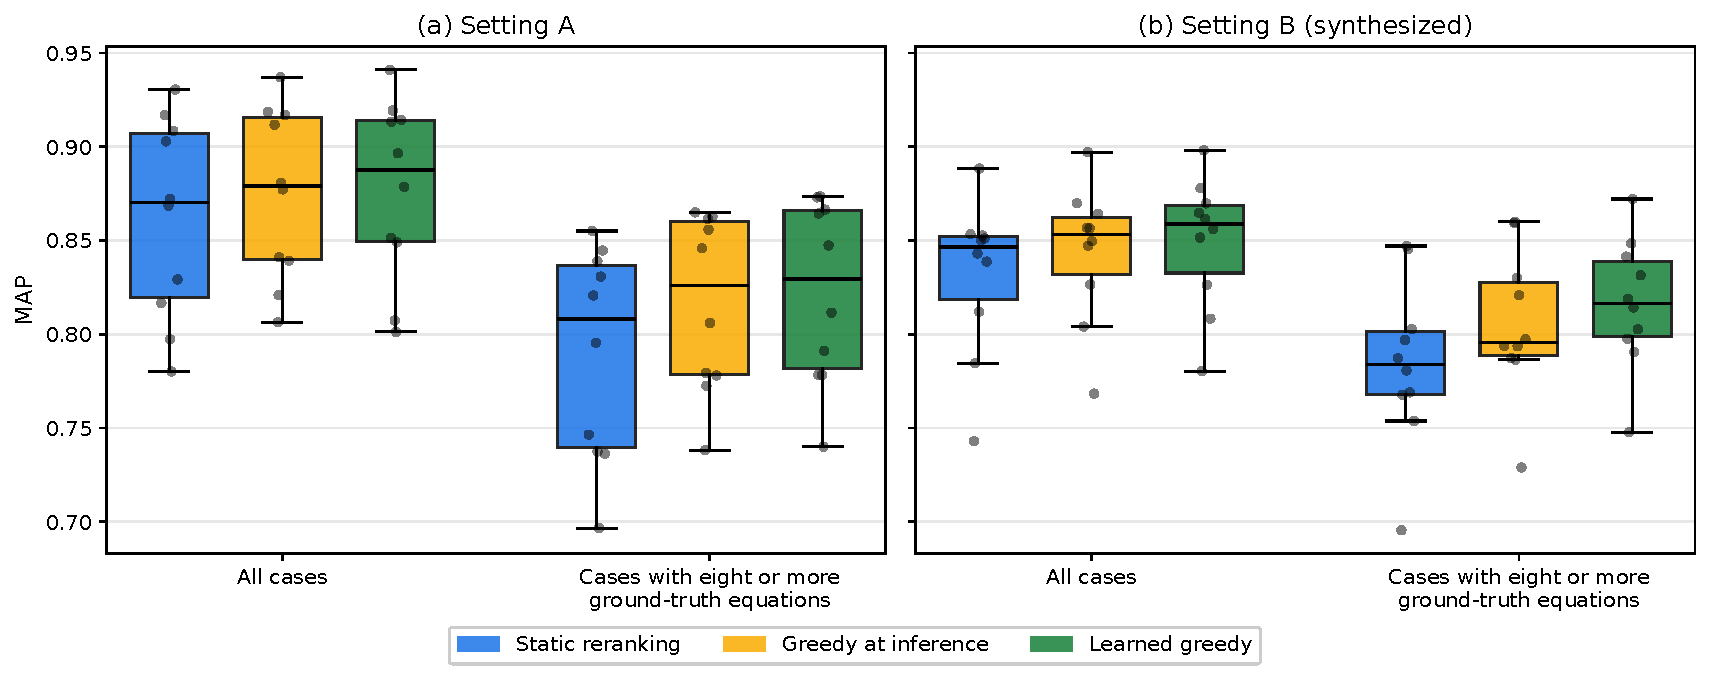
\includegraphics[width=\linewidth]{figures/fig_greedy_3way.pdf}
\caption{MAP of the three selection strategies in (a) Setting~A and (b) Setting~B, on all cases
and on the cases with eight or more ground-truth equations. Boxes show the 10 splits.}
\label{fig:greedy}
\end{figure}
